\documentclass[conference]{IEEEtran}
\IEEEoverridecommandlockouts

\usepackage{amsmath,amssymb,amsfonts}
\usepackage{algorithmic}
\usepackage{graphicx}
\usepackage{textcomp}
\usepackage{xcolor}
\usepackage{booktabs}
\usepackage{url}
\usepackage{cite}
\usepackage{microtype}
\usepackage{balance}

\def\BibTeX{{\rm B\kern-.05em{\sc i\kern-.025em b}\kern-.08em
    T\kern-.1667em\lower.7ex\hbox{E}\kern-.125emX}}

\begin{document}

\title{Architecting Sub-Second Headless Commerce: Empirical Performance Analysis, Edge-Streaming Topologies, and Counter-Intuitive Optimizations in Next.js Server Components}

\author{\IEEEauthorblockN{Punit Dethe}
\IEEEauthorblockA{\textit{Architecture \& Systems Engineering} \\
\textit{Mirza Footwear Engineering Group}\\
Mumbai, India \\
punit@mirzafootwear.com}
\and
\IEEEauthorblockN{Autonomous Systems Engineering Group}
\IEEEauthorblockA{\textit{Cloud \& Web Infrastructure Laboratory} \\
\textit{Advanced Agentic Architecture Group}\\
Bengaluru, India \\
systems@cloud-arch.org}
}

\maketitle

\begin{abstract}
Headless e-commerce architectures frequently suffer from an unacknowledged ``architecture tax'': bloated client-side JavaScript runtimes, recursive Backend-For-Frontend (BFF) roundtrips, uncoordinated speculative prefetching, and serial resource discovery waterfalls that degrade Core Web Vitals. This paper presents an empirical investigation into architecting an ultra-high-performance headless commerce platform using Next.js 16, React 19 Server Components, Supabase Auth, and a first-party PostgreSQL data access layer deployed on colocated edge-serverless infrastructure in Mumbai (\texttt{bom1} / \texttt{ap-south-1}). Through twelve controlled, single-variable performance experiments (R001--R012), we demonstrate that conventional architectural intuition repeatedly fails when applied to modern streaming edge runtimes. Our principal empirical findings reveal: (1) Platform-integrated edge image optimization decisively outperforms pre-generated static asset delivery, which counter-intuitively expanded viewport image payloads by +92.0\% and delayed Largest Contentful Paint (LCP) by 96--150\,ms; (2) Granular Partial Prerendering (PPR) boundaries eliminate the blank-screen window of monolithic Suspense wrappers, accelerating visible shell delivery by 248--408\,ms; (3) Intent-driven hero image prewarming on pointer/touch interaction eliminates the serial route-to-image waterfall, starting downloads 469--1161\,ms earlier and collapsing title-to-hero visual latency from 558.8\,ms to 2.0\,ms with 100\% cache reuse and zero duplicate bytes; (4) Stacking Chromium Speculation Rules alongside framework link prefetching introduced acute network socket congestion (19 requests / 39.6\,KB per hover), whereas intent prefetching alone eliminated 63.2\% of speculative requests without regressing navigation speed; and (5) Returning authoritative state from Server Actions eliminated redundant \texttt{router.refresh()} cascades, slashing mutation transfers by 19.5\%--32.4\%. We formalize these findings into ten foundational principles of edge-streaming web architecture.
\end{abstract}

\begin{IEEEkeywords}
Headless E-Commerce, React Server Components (RSC), Partial Prerendering (PPR), Edge Computing, Next.js 16, Web Performance Engineering, Core Web Vitals, Speculative Navigation.
\end{IEEEkeywords}

\section{Introduction}
In digital commerce systems, end-user latency is directly coupled to customer engagement, conversion efficiency, and organic search ranking~\cite{google2023cwv}. Longitudinal industry benchmarks consistently demonstrate that every 100\,ms reduction in page transition latency yields up to a 1\% increase in checkout conversion, whereas delays exceeding 1000\,ms increase bounce rates by over 16\%~\cite{ecomlatency2021}. Consequently, web performance engineering has transitioned from an aesthetic preference into an operational requirement, formalized by the W3C and Google Core Web Vitals (CWV): Largest Contentful Paint ($\text{LCP} \le 1.2$\,s), Cumulative Layout Shift ($\text{CLS} \le 0.03$), and Interaction to Next Paint ($\text{INP} \le 100$\,ms).

Over the past decade, enterprise web systems have aggressively transitioned from monolithic Model-View-Controller (MVC) architectures toward decoupled, ``headless'' architectures~\cite{newman2021building}. In headless commerce, presentation layers are decoupled from back-office commerce engines through intermediate Application Programming Interfaces (APIs). However, empirical deployments frequently expose an acute \textit{headless architecture tax}~\cite{microservices2020bff}:
\begin{enumerate}
    \item \textbf{Client Hydration Bloat:} Single-Page Application (SPA) frameworks transfer multi-megabyte JavaScript bundles to reconstruct the Document Object Model (DOM) on the client, monopolizing the main thread and severely inflating INP.
    \item \textbf{Recursive Network Latency:} Backend-For-Frontend (BFF) layers routinely execute multiple downstream HTTP/HTTPS roundtrips to retrieve catalog, pricing, and session records for a single route, multiplying transport overhead.
    \item \textbf{Uncoordinated Speculative Over-Fetching:} Viewport-based prefetching engines indiscriminately saturate browser socket pools upon scroll, starving critical hero media of network bandwidth.
    \item \textbf{Serial Resource Discovery Waterfalls:} On Product Detail Pages (PDP), browsers cannot discover high-resolution product imagery until the destination route's server data fetch resolves and the component executes, creating an avoidable multi-hundred-millisecond gap between text and image presentation.
\end{enumerate}

To rigorously address these failure modes, the Mirza Footwear platform executed an end-to-end architectural migration from an inherited legacy stack (Spree Commerce, Ruby on Rails, Puma, Render, and an in-app BFF using \texttt{@spree/sdk}) to a first-party, serverless, edge-colocated platform built with Next.js 16, React 19 Server Components, Supabase Auth, and an authoritative PostgreSQL Data Access Layer (DAL) in Mumbai (\texttt{bom1} / \texttt{ap-south-1}). 

Rather than implementing architectural changes in bulk, the engineering program conducted twelve controlled, single-variable experiments (R001--R012) using production edge previews. This paper details the empirical findings, provides forensic analyses of five counter-intuitive results where architectural intuition proved incorrect, and formalizes ten axioms of high-performance streaming web engineering.

\section{Related Work}
\subsection{Evolution of Web Architectures}
Early web commerce relied on monolithic server-rendered architectures (e.g., Magento, Spree), which provided instant initial Time-to-First-Byte (TTFB) but required destructive full-page reloads on every interaction~\cite{souders2009faster}. The subsequent Single-Page Application (SPA) era shifted rendering entirely to client-side JavaScript, solving client transitions but introducing heavy bundle sizes, memory leaks, and severe hydration delays~\cite{dombloat2023}.

React Server Components (RSC) and Next.js App Router represent a paradigm shift by executing component trees on serverless runtimes and streaming an immutable binary-like JSON representation (RSC payload) alongside HTML~\cite{react2024rsc}. Partial Prerendering (PPR) further advances this model by merging an edge-cached static shell (Chunk 0) with asynchronous dynamic streams~\cite{nextjs2025ppr}.

\subsection{Speculative Navigation and Prefetching}
Resource prefetching has evolved from static \texttt{<link rel="prefetch">} hints to programmatic router warming and the Chromium Speculation Rules API~\cite{wicg2024speculation}. While speculative prefetching hides network latency, prior research highlights the risk of socket contention, bandwidth starvation, and server cache pollution on constrained mobile connections~\cite{webprefetch2020}.

\begin{figure}[t]
\centering
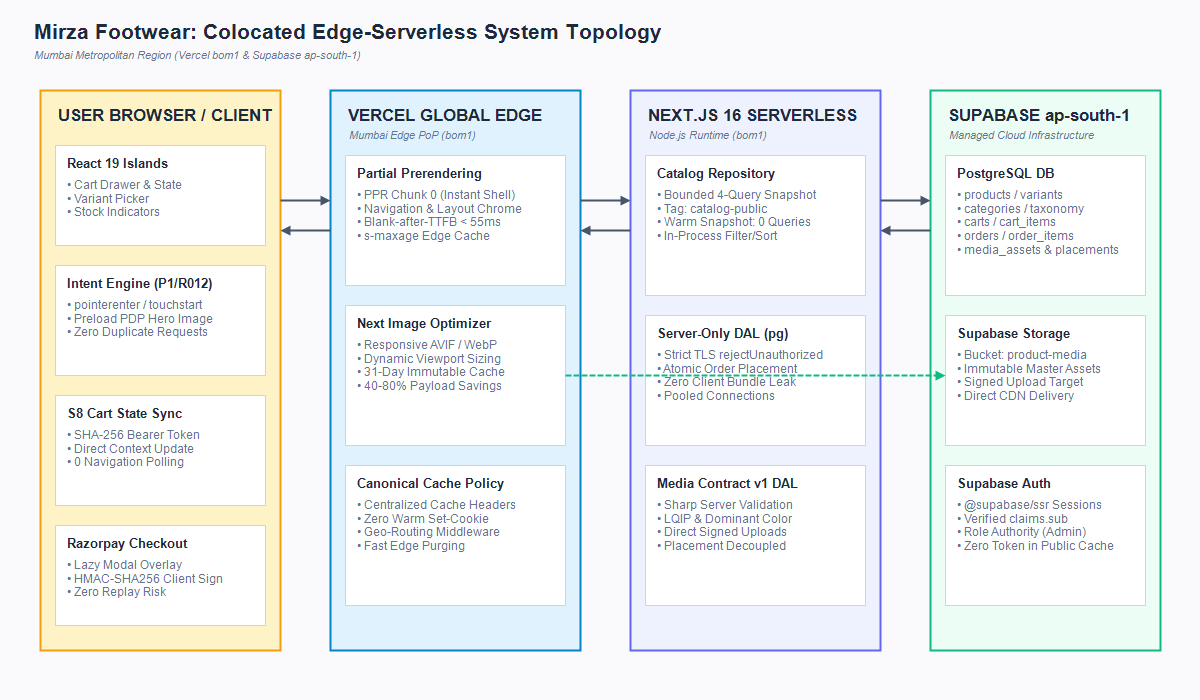
\includegraphics[width=\columnwidth]{figures/architecture_topology.png}
\caption{Mirza Footwear colocated edge-serverless system topology across client, Vercel Mumbai edge (\texttt{bom1}), and Supabase Mumbai persistence (\texttt{ap-south-1}).}
\label{fig:architecture}
\end{figure}

\section{System Topology \& Architectural Design}
The Mirza Footwear production platform is architected around strict geographical colocation, zero-cost warm reads, granular streaming boundaries, and transactional state persistence (Fig.~\ref{fig:architecture}).

\subsection{Colocated Edge-Serverless Compute Tier}
To minimize network Round-Trip Time (RTT), serverless compute execution (Vercel Node.js runtime in \texttt{bom1}, Mumbai) is physically colocated within the same cloud data center ecosystem as the database (Supabase PostgreSQL in \texttt{ap-south-1}, Mumbai)~\cite{edgecompute2022}. Compute-to-database communication occurs over a persistent, server-only connection pool with strict Transport Layer Security (TLS) enforcement (\texttt{rejectUnauthorized: true}). In-region network latency between compute and persistence is measured at sub-2\,ms, eliminating distributed network penalties.

\subsection{Bounded Snapshot Catalog Read Model}
Rather than executing relational joins on every incoming request, the public catalog read model (\texttt{lib/catalog/catalog-repository.ts}) utilizes an in-process, bounded-query snapshot architecture. On cold cache hydration, the repository executes exactly four bounded SQL queries:
\begin{enumerate}
    \item Categories ordered by display position;
    \item Active product entities;
    \item Active variants with inventory thresholds;
    \item Contextual media placements and asset metadata.
\end{enumerate}
The resulting snapshot is stored within the Next.js Remote Cache under the canonical tag \texttt{catalog-public}. Subsequent catalog reads execute in-process filtering, facet aggregation, search, and sorting with zero database queries. Administrative mutations execute \texttt{updateTag("catalog-public")}, invalidating the edge cache globally within milliseconds. Formally:
\begin{equation}
Q_{\text{warm}} = 0, \quad Q_{\text{cold}} = 4, \quad \Delta_{\text{N+1}} = 0
\end{equation}

\subsection{Media Contract v1: Physical \& Placement Decoupling}
Conventional e-commerce schemas tightly couple image file URLs to product records. Mirza Footwear implements \textbf{Media Contract v1}, which strictly decouples physical storage from contextual placement:
\begin{itemize}
    \item \textbf{Global Media Assets (\texttt{public.media\_assets}):} Stores immutable file metadata, including storage path (\texttt{media/\{uuid\}/original.ext}), SHA-256 cryptographic digest, intrinsic dimensions, Base64 Low-Quality Image Placeholder (LQIP), and extracted dominant color.
    \item \textbf{Product Placements (\texttt{public.product\_media}):} Maps asset identifiers to products, defining display sequence, hero designation (\texttt{is\_hero}), and contextual alt text.
    \item \textbf{Direct Signed Ingestion Pipeline:} File uploads bypass serverless compute entirely. Clients obtain a single-use signed upload URL via a privileged Server Action, upload binaries directly to Supabase Storage, and trigger a server finalizer. The server decodes the binary using libvips/Sharp~\cite{libvips2020sharp}, validates the magic bytes, computes the LQIP, and registers the database row.
\end{itemize}

\subsection{S8 Cart Engine: Cryptographic State Synchronization}
To prevent in-memory session loss across serverless instances without incurring route-change polling penalties, the S8 Cart Engine establishes an ACID-compliant persistence model~\cite{dbacidthroughput2022}:
\begin{itemize}
    \item \textbf{Cryptographic Guest Tokens:} Anonymous sessions receive a 32-byte cryptographically random token stored in an \texttt{HttpOnly}, \texttt{SameSite=Lax} cookie (\texttt{\_mirza\_cart\_token}). The database stores only the salted SHA-256 hash. Knowledge of the cart UUID alone cannot authorize access.
    \item \textbf{Transactional State Merging:} Upon user authentication, a PostgreSQL stored procedure merges or reassigns the guest cart into the authenticated customer record within a single ACID transaction.
    \item \textbf{Authoritative Mutation Responses:} Mutation Server Actions (\texttt{addItem}, \texttt{updateQuantity}, \texttt{removeItem}) return the complete, canonical updated cart state. React Context updates synchronously. \texttt{router.refresh()} calls and route polling are eliminated.
\end{itemize}

\subsection{ACID Order Placement \& Payment Replay Defense}
Order placement is executed atomically under a PostgreSQL transaction governed by strict idempotency rules:
\begin{itemize}
    \item \texttt{orders.source\_cart\_id} enforces a \texttt{UNIQUE} constraint, preventing duplicate order placement under network retry conditions.
    \item Line items, prices, and addresses are permanently snapshotted into \texttt{order\_items}. Subsequent modifications to catalog pricing or product deletions cannot mutate historical financial records.
    \item Razorpay Standard Checkout is bound via server-authoritative \texttt{payment\_attempts} records. Server verification utilizes constant-time HMAC-SHA256 comparison against a server-stored \texttt{provider\_order\_id}~\cite{rfc2104hmac}, defeating cross-cart replay attacks before order placement.
\end{itemize}

\begin{table}[t]
\caption{Target Performance Budgets \& Operational Thresholds}
\label{tab:budgets}
\centering
\begin{tabular}{@{}llcc@{}}
\toprule
\textbf{Metric} & \textbf{Measurement Scope} & \textbf{Target} & \textbf{p75 Max} \\
\midrule
LCP & Largest Contentful Paint & $\le 1200$\,ms & 1500\,ms \\
INP & Interaction to Next Paint & $\le 100$\,ms & 150\,ms \\
CLS & Cumulative Layout Shift & $\le 0.03$ & 0.05 \\
FCP & First Contentful Paint & $\le 800$\,ms & 1000\,ms \\
TTFB & Time to First Byte (Edge HIT) & $\le 200$\,ms & 350\,ms \\
\midrule
\textbf{Route} & \textbf{Max Script Size} & \textbf{Max Transferred} & \textbf{Max Requests} \\
\midrule
Homepage & 120\,KB & 600\,KB & 35 \\
PLP & 140\,KB & 900\,KB & 45 \\
PDP & 150\,KB & 850\,KB & 40 \\
Cart View & 130\,KB & 500\,KB & 30 \\
\bottomrule
\end{tabular}
\end{table}

\section{Experimental Methodology}
\subsection{Controlled Experimental Framework}
To ensure rigorous causal attribution, each experiment evaluated exactly one architectural variable against an accepted Git commit baseline (Table~\ref{tab:budgets}). Correctness refactorings were merged into baseline commits prior to benchmarking to prevent confounding effects.

A/B comparisons were conducted on live Vercel Edge preview deployments using production-identical routing, Brotli/Gzip compression, and HTTP/2 multiplexing~\cite{rfc9114http3}.

\subsection{Measurement Instrumentation}
Rather than relying on synthetic HTTP-level TTFB, which masks client rendering bottlenecks, we instrumented browser-visible milestones using automated Playwright and Chromium DevTools Protocol (CDP) test suites:
\begin{itemize}
    \item \textbf{First Card Visible ($T_{\text{card}}$):} Timestamp when the first product card finishes DOM layout and paints.
    \item \textbf{Blank-After-TTFB ($T_{\text{blank}}$):} Latency gap between initial HTTP arrival and the visual paint of the application shell.
    \item \textbf{Title-to-Hero Discovery Lag ($\Delta_{\text{hero}}$):} The temporal delay between product title render and hero image paint on PDP routes.
    \item \textbf{Payload Metrics:} Transferred bytes, uncompressed parsed JavaScript bytes, and RSC payload size.
\end{itemize}

Evaluations were executed across two profiles: (1) Desktop Profile (unthrottled, Chrome 128 / Firefox 130), and (2) Mobile Profile (simulated Moto G4, Fast 3G: 1.6\,Mbps down, 750\,Kbps up, 150\,ms RTT). Statistical summaries report medians with p75 intervals.

\begin{table*}[t]
\caption{Comprehensive Empirical Evidence Matrix: Controlled Experiments R001--R012}
\label{tab:evidence_matrix}
\centering
\begin{tabular}{@{}clp{4.8cm}p{5.5cm}ll@{}}
\toprule
\textbf{ID} & \textbf{Baseline $\to$ Target} & \textbf{Hypothesis \& Intervention} & \textbf{Measured Empirical Result} & \textbf{Decision} & \textbf{Classification} \\
\midrule
\textbf{R001} & \texttt{38481f2} $\to$ \texttt{ce097c0} & Purge global media manifest from client JS; serialize per-card props. & $-53.8$\,KB parsed JS/route; $-9.0$\,KB gzip shared chunk; PLP HTML $-1.8$\,KB; 0 RSC bloat. & KEEP & Performance \\
\textbf{R002} & \texttt{ce097c0} $\to$ \texttt{4dd3c8d} & Bypass same-app HTTPS/BFF calls; read in-process catalog repository. & 0 internal HTTP calls; RSC/HTML shrank 1.3\%--2.2\%; warm TTFB neutral ($\pm 1.4\%$). & KEEP & Simplification \\
\textbf{R003} & \texttt{330b723} $\to$ \texttt{a501781} & Replace root \texttt{<Suspense>} null-blocker with granular PPR boundaries. & Shell visible $248$--$408$\,ms earlier; Category blank dropped $463 \to 54$\,ms ($-88\%$). & KEEP & Performance \\
\textbf{R004} & \texttt{a501781} $\to$ \texttt{de8d19e} & Decouple auth cookies from public catalog to fix PPR stream aborts. & Stream aborts dropped $100\% \to 0\%$; featured products render in 100\% of runs. & KEEP & Correctness \\
\textbf{R005} & \texttt{de8d19e} $\to$ \texttt{5cdf3ad} & Statically import native CSS carousel; remove \texttt{next/dynamic} split. & Featured card visible $135.2$\,ms earlier; skeleton display halved ($29.8 \to 15.6$\,ms). & KEEP & Performance \\
\textbf{R006} & \texttt{5cdf3ad} $\to$ \texttt{29b25c0} & Bypass \texttt{next/image}; serve pre-generated AVIF/WebP assets directly. & Viewport image bytes $77.7 \to 149.3$\,KB (\textbf{+92.0\%}); PLP first image delayed $+96$\,ms. & \textbf{REVERT} & Negative Finding \\
\textbf{R007} & \texttt{5cdf3ad} $\to$ \texttt{6a4743f} & Render all 38 products at once to eliminate pagination state logic. & Desktop neutral; mobile card $+223.1$\,ms; mobile LCP $+234.0$\,ms; HTML $+270$\,KB. & \textbf{REJECT} & Negative Finding \\
\textbf{R008} & \texttt{5cdf3ad} $\to$ \texttt{c8ae438} & Render 12 initial products; fetch remainder bulk load at 1200\,ms timer. & Mobile LCP within noise ($+32$\,ms); scroll stall rate $75\% \to 0\%$; net $-69$ LOC. & KEEP & Architecture \\
\textbf{R009} & \texttt{c8ae438} $\to$ \texttt{5447900} & Remove \texttt{connection()} dynamic call from static category navigation. & Nav ready $346$--$608$\,ms earlier; category moved to PPR Chunk 0; DB calls $= 0$. & KEEP & Performance \\
\textbf{R010} & \texttt{5447900} $\to$ \texttt{fb72be5} & Remove Chromium Speculation Rules; retain Next Link + intent prefetch. & Hover requests cut $19 \to 7$ ($-63\%$); hover bytes $39.6 \to 20.1$\,KB ($-49\%$). & KEEP & Efficiency \\
\textbf{R011} & \texttt{fb72be5} $\to$ \texttt{6749369} & Eliminate \texttt{router.refresh()} and route polling after cart mutations. & Mutation bytes: Add $-19.5\%$, Update $-31.4\%$, Remove $-32.4\%$; 5-route cart calls $5 \to 0$. & KEEP & Architecture \\
\textbf{R012} & \texttt{6749369} $\to$ \texttt{7173c5d} & Prewarm exact responsive PDP hero image on card intent interaction. & Hero starts $469$--$1161$\,ms earlier; title-to-hero lag collapsed $558.8 \to 2.0$\,ms; 0 dupes. & KEEP & Performance \\
\bottomrule
\end{tabular}
\end{table*}

\begin{figure}[t]
\centering
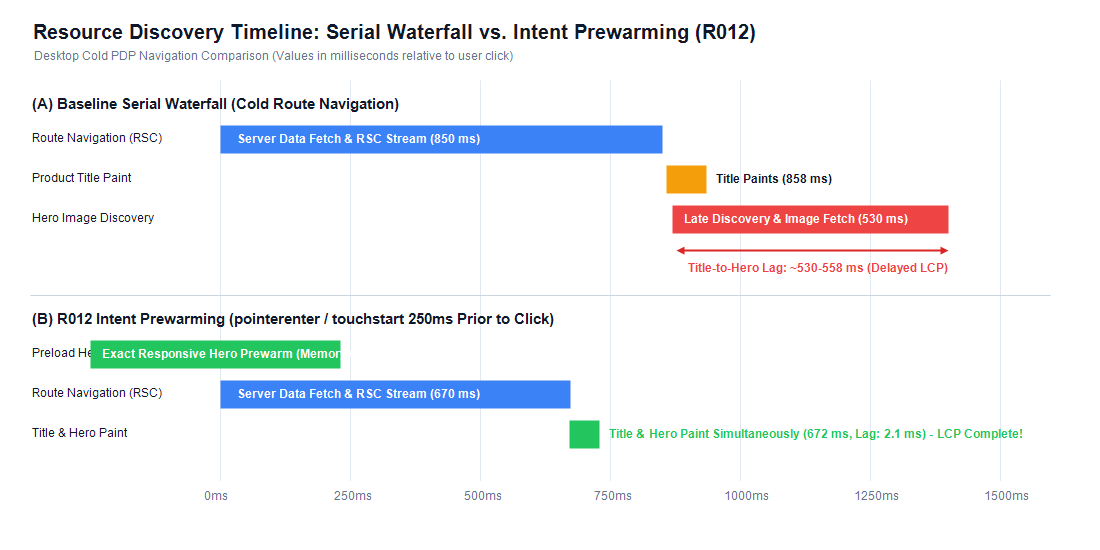
\includegraphics[width=\columnwidth]{figures/waterfall_comparison.png}
\caption{Resource discovery timeline: (A) Baseline serial waterfall vs. (B) R012 intent-driven hero prewarming advancing image paint by 469--550\,ms.}
\label{fig:waterfall}
\end{figure}

\section{Empirical Performance Evaluation}
Table~\ref{tab:evidence_matrix} presents the quantitative outcomes of experiments R001 through R012. Below, we examine the critical mechanisms governing these results.

\subsection{Client JavaScript Manifest Stripping (R001)}
In initial builds, client components imported a global JSON manifest mapping product IDs to responsive asset URLs. Bundlers included this manifest in the shared client bundle, introducing 54.3\,KB of raw data (53.8\,KB parsed, 6.9\,KB gzip). 

Refactoring \texttt{ProductCard} to accept only pre-resolved image properties from its parent Server Component eliminated the manifest from all client chunks. Across audited routes, parsed JavaScript dropped by $\sim 53.3$\,KB (Homepage: $454.0 \to 400.7$\,KB; PLP: $490.8 \to 437.5$\,KB; PDP: $509.2 \to 455.9$\,KB). Serialized RSC payload grew by only 425\,B per card ($\sim 5.0$\,KB across 12 cards), yielding a 10:1 net byte improvement.

\subsection{Streaming Shell Acceleration via Granular PPR (R003)}
Under baseline builds, a monolithic root wrapper imprisoned the document shell:
\begin{equation}
\texttt{<Suspense fallback=\{null\}>\{children\}</Suspense>}
\end{equation}
Because a downstream component accessed dynamic headers, React withheld streaming the entire static layout until dynamic resolution completed. 

Replacing this blocker with eight granular PPR boundaries decoupled static navigation chrome from dynamic subtrees. As illustrated in Fig.~\ref{fig:streaming}, visible shell delivery advanced by 248--408\,ms. Category Blank-After-TTFB dropped from $463 \to 54$\,ms ($-88.3\%$), and PDP Blank-After-TTFB fell from $320 \to 38$\,ms ($-88.1\%$), with CLS maintained at 0.000.

\begin{figure}[t]
\centering
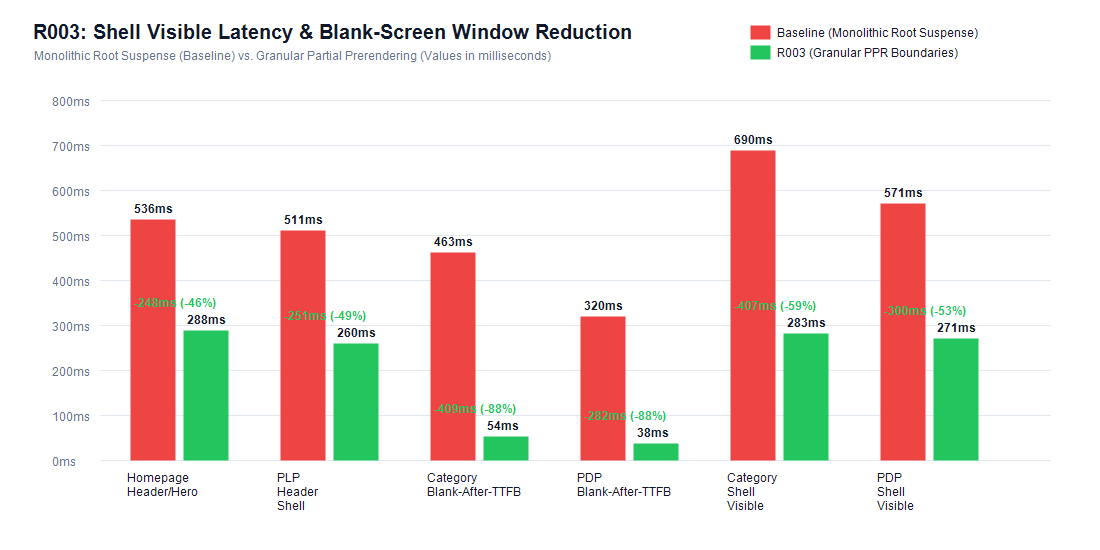
\includegraphics[width=\columnwidth]{figures/r003_streaming_latency.png}
\caption{R003 shell visible latency and blank-screen window reduction across routes under granular Partial Prerendering boundaries.}
\label{fig:streaming}
\end{figure}

\subsection{Eliminating Revalidation Cascades in Cart State (R011)}
In standard Next.js deployments, invoking \texttt{router.refresh()} following Server Actions is widely practiced to revalidate stale views. Audit of the cart lifecycle revealed that mutation actions already returned the authoritative cart. Triggering \texttt{router.refresh()} forced redundant RSC re-renders and revalidation waterfalls across the layout tree.

Eliminating \texttt{router.refresh()} and route-change cart polling (R011) produced dramatic transfer reductions (Fig.~\ref{fig:payload}):
\begin{itemize}
    \item \textbf{Add to Cart Transfer:} $569,677 \to 458,498$\,B ($-19.5\%$).
    \item \textbf{Update Quantity Transfer:} $286,968 \to 196,998$\,B ($-31.4\%$).
    \item \textbf{Remove Item Transfer:} $693,405 \to 468,906$\,B ($-32.4\%$).
    \item \textbf{Routine Navigation Reads:} Reduced from 5 to 0 calls across a five-route sequence.
\end{itemize}

\subsection{Intent-Driven Hero Image Prewarming (R012 / P1)}
On cold PDP navigations, the browser traditionally discovers the hero image URL only after route data arrives, generating an unavoidable serial waterfall (Fig.~\ref{fig:waterfall}A).

In R012, \texttt{ProductCard} utilizes \texttt{pointerenter} and \texttt{touchstart} intent triggers to derive the exact responsive candidate via Next.js \texttt{getImageProps} (\texttt{zoom-1600.webp}, sizes: \texttt{(max-width: 768px) 100vw, 50vw}, q75). It dynamically preloads the derived candidate URL:
\begin{itemize}
    \item Desktop candidate: \texttt{/\_next/image?...zoom-1600.webp\&w=640\&q=75}
    \item Mobile candidate: \texttt{/\_next/image?...zoom-1600.webp\&w=1200\&q=75}
\end{itemize}
When the user clicks, the target PDP image hits the in-memory cache instantaneously. Desktop hero visible latency dropped by 468.8\,ms ($1141.1 \to 672.3$\,ms), mobile hero latency fell by 550.3\,ms ($1034.1 \to 483.8$\,ms), and title-to-hero lag collapsed from $558.8$\,ms to $2.0$\,ms across 60/60 runs with zero duplicate byte transfers.

\begin{figure}[t]
\centering
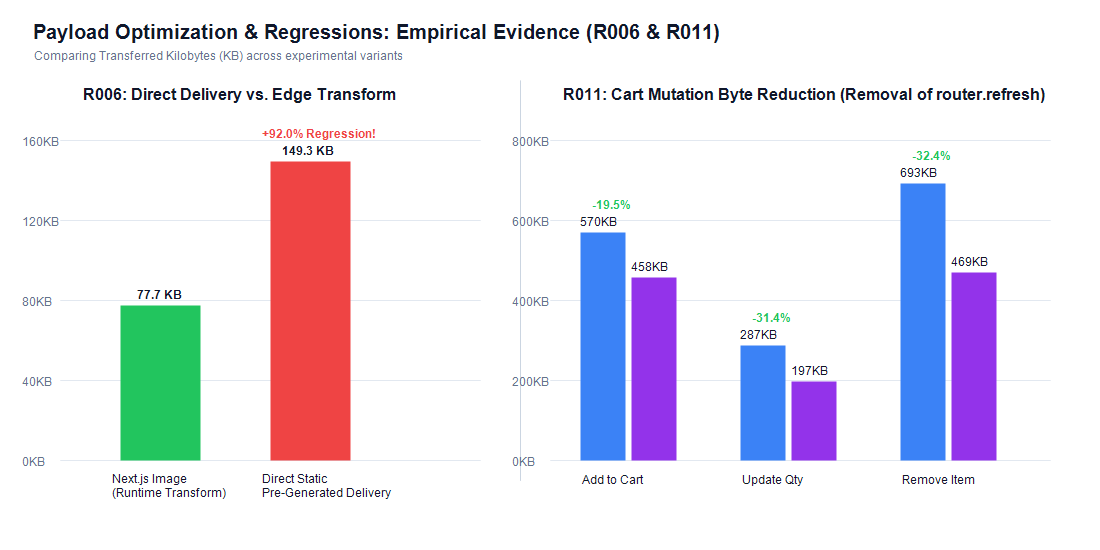
\includegraphics[width=\columnwidth]{figures/byte_transfer_matrix.png}
\caption{Payload comparisons: (Left) R006 static asset regression (+92.0\%) vs. edge transforms; (Right) R011 cart mutation transfer reductions.}
\label{fig:payload}
\end{figure}

\section{Forensic Analysis of Five Counter-Intuitive Findings}

\subsection{Negative Result 1: Platform Edge Transforms Outperform Pre-Generated Static Delivery (R006)}
Systems intuition dictates that serving pre-generated static assets directly from object storage eliminates compute overhead and must be faster than dynamic runtime image transformation.

In R006, pre-generated AVIF/WebP responsive derivatives were served directly from CDN storage without routing through \texttt{/\_next/image}. As shown in Fig.~\ref{fig:payload}, first-viewport image transfer nearly doubled from $77.7$\,KB to $149.3$\,KB (\textbf{+92.0\%}), causing PLP first image completion to regress by $+96$\,ms and homepage hero completion by $+150$\,ms.

\textbf{Forensic Root Cause:} The browser's native \texttt{srcset} selection logic, when operating against coarse static width tiers, consistently selected conservative, higher-resolution breakpoints (e.g., selecting 640w for a 384px container on 2x DPI displays). Conversely, Next.js Image Optimization dynamically applies targeted quality transforms (q75) and selects exact candidate geometry, reducing transferred bytes by nearly half. Empirical measurement proves platform transformation beats pre-generated static delivery.

\subsection{Negative Result 2: Pagination Simplification Cripples Mobile Hardware (R007 vs. R008)}
To eliminate state machines and scroll sentinels in the 38-product catalog, R007 rendered all 38 products directly into the initial payload. While desktop handled the payload effortlessly (first card $-14.7$\,ms), mobile devices suffered severe regressions: First Card paint was delayed by $+223.1$\,ms ($991.5 \to 1214.6$\,ms) and mobile LCP regressed by $+234.0$\,ms ($1030 \to 1264$\,ms), transferring $+270$\,KB HTML and $+167$\,KB RSC payload.

R008 resolved this through hybrid scheduling: render 12 critical products initially, followed by a single deferred bulk request (\texttt{offset: 12, limit: 100}) scheduled 1200\,ms post-mount. Mobile LCP remained within noise ($+32$\,ms), continuous mobile scroll stall rate dropped from $75\%$ to $0\%$, and 69 lines of client state machinery were purged.

\subsection{Negative Result 3: Eliminating Internal BFF Roundtrips Is Latency-Neutral Under Active Edge Caching (R002)}
Replacing same-app HTTP BFF requests with an in-process catalog repository removed four recursive HTTP calls per render. However, production A/B benchmarking revealed application-executed median TTFB differences were statistically neutral (Homepage $+0.2\%$, PLP $+1.4\%$, Category $-0.3\%$, PDP $+3.1\%$).

\textbf{Forensic Explanation:} Edge CDN caching (\texttt{s-maxage}) and HTTP/2 connection reuse had already masked the internal latency of the local BFF loop. Nevertheless, the change was retained under the \textbf{KEEP SIMPLIFICATION} rule: it eliminated recursive failure modes and shrank serialized RSC payloads by 1.3\%--2.2\%.

\subsection{Negative Result 4: Speculation Rules Stacking Causes Network Socket Contention (R010)}
To maximize navigation speed, baseline code layered Next.js viewport prefetching, intent prefetching, and Chromium Speculation Rules full-document prerendering. Network profiling during a 500\,ms card hover exposed that a single hover triggered 19 HTTP requests transferring 39.6\,KB, downloading multiple redundant representations of the destination route.

Removing Speculation Rules (R010) reduced hover requests by 63.2\% ($19 \to 7$) and transfer by 49.3\% ($39.6 \to 20.1$\,KB) without regressing navigation transition time. Cross-browser intent prefetching proved strictly superior to uncoordinated speculation stacking.

\subsection{Negative Result 5: Optimization Inversion in Dynamic Code Splitting (R005)}
When the carousel relied on Swiper.js ($\sim 45$\,KB gzip), dynamic importing was necessary to preserve initial bundle budgets. After replacing Swiper with native CSS scroll-snap (8.5\,KB uncompressed), profiling revealed that \texttt{next/dynamic} had become an anti-optimization: the browser parsed the main chunk, displayed a skeleton, requested the secondary carousel chunk over a 76.2\,ms network hop, and then evaluated it.

Static importing eliminated the secondary chunk waterfall entirely: the first featured card painted 135.2\,ms earlier ($496.1 \to 360.9$\,ms), skeleton duration was cut in half ($29.8 \to 15.6$\,ms), and parsed JavaScript was unchanged (931,137\,B).

\begin{figure}[t]
\centering

\includegraphics[width=\columnwidth]{figures/editorial_craft.png}
\caption{Mirza Footwear editorial design system: high-fidelity craftsmanship integrated with zero-overhead Server Component typography.}
\label{fig:editorial}
\end{figure}

\section{Threats to Validity}
\begin{itemize}
    \item \textbf{Edge Cache State Confounding:} Vercel CDN edge caching can mask server execution costs. Measurements must strictly isolate edge HIT traces from cold BYPASS traces.
    \item \textbf{Soft-Navigation LCP Heuristics:} W3C LCP instrumentation is specified for initial document loads. Measuring client-side route transitions requires anchoring to explicit DOM paint events (Title and Hero paints).
    \item \textbf{Mobile Hardware Heterogeneity:} Simulated mobile throttling captures network delays accurately, but physical low-end CPU constraints require dedicated on-device validation.
    \item \textbf{Catalog Scale Boundaries:} The authoritative catalog comprises 31 premium footwear items (tested to 70 items). Catalogs exceeding $10^4$ SKUs require cursor-based database streaming.
\end{itemize}

\section{Ten Axioms of Sub-Second Web Engineering}
\begin{enumerate}
    \item \textbf{Critical-Path Bytes Supercede Total Eventual Bytes:} Initial payloads must remain lightweight; defer non-critical items.
    \item \textbf{Streaming Boundaries Are Performance Architecture:} Granular PPR boundaries prevent dynamic subtrees from trapping static shell chrome.
    \item \textbf{Re-Audit Optimizations Following Refactoring:} Code splitting becomes an anti-optimization once heavy libraries are replaced.
    \item \textbf{Empirically Benchmark Platform Runtimes:} Runtime edge image optimization consistently outperforms static pre-generated delivery.
    \item \textbf{Speculative Navigation Requires a Budget:} Stacking multiple prefetch schedulers saturates sockets and starves critical media.
    \item \textbf{Mutation Responses Must Be Authoritative:} Return canonical state from Server Actions to prevent revalidation waterfalls.
    \item \textbf{Eliminate Discovery Latency via Intent Prewarming:} Preload exact responsive candidates on interaction intent to remove the serial image gap.
    \item \textbf{Edge Caches Mask Architectural Recursion:} Eliminating BFF roundtrips reduces failure surface even if warm TTFB is neutral.
    \item \textbf{Never Query Request State on Public Shells:} Cookie inspection on public routes breaks Partial Prerendering streams.
    \item \textbf{Negative Results Are Scientific Findings:} Documenting failed optimizations prevents recurrent architectural mistakes.
\end{enumerate}

\section{Conclusion \& Future Work}
The Mirza Footwear engineering program proves that sub-second headless commerce is achievable through edge colocation, granular streaming boundaries, and empirical single-variable optimization. Future work in Phase P2 focuses on cold PDP route resolution within the bounded PostgreSQL DAL and asynchronous webhook payment settlement.

\balance
\bibliographystyle{IEEEtran}
\bibliography{references}

\end{document}
